\subsection{Electronic chain linearity}

In order to prepare the data acquistion system, the entire electronical chain
was tested beforehand. In fact it is crucial that the response of each
electronic device used behaves linearly, as the information about the energy
of the incident particle must be univocally extracted at the end of the chain.

\begin{figure}[h]
  \centering
  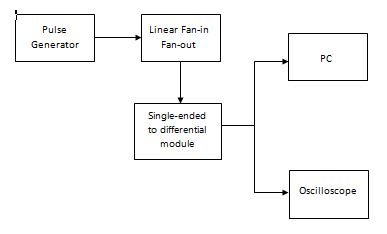
\includegraphics[scale=.5]{img/electronic_chain_diagram.JPG}
  \caption{The electronic chain}
  \label{chain}
\end{figure}

The setup used is shown in Fig.~\ref{chain}. The output of a pulse generator (\num{100}ns square pulse of variable amplitude) is fed into a Fan-in Fan-out which reproduces the same signal for 12 channels, this signals are given in input to a single-ended to differential amplifier custom board, in order to do this a cable was made.
The output of the board as seen from the oscilloscope is shown in Fig.~\ref{osc}. The shape of the rising edge of this signal will be sampled during the acquisition from the detector in order to perform PSA on each event.


\begin{figure}[h]
  \centering
  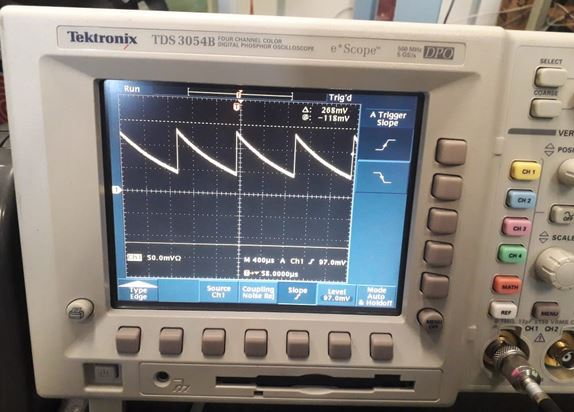
\includegraphics[scale=.35]{img/test_signal_oscilloscope.JPG}
  \caption{The output signal from the differential amplifier board, as seen on the oscilloscope.}
  \label{osc}
\end{figure}

From the board the signal is given to a 100 MHz 14-bit resolution digitizer throught a MDR-26 connector
At the signal is the applied, with an FPGA, a trapezoidal filter with its charateristics \emph{risetime} and \emph{flat top} width parameters (Moving Windows Analysis) [INSERT REF. DESCRIBING THIS METHOD], this step is crucial because because the height of the peak from the differential amplifier board will be directly proportional to the energy of the incident particle in the detector.
The height trapezoidal filter with the right parameters then gives the information on the intensity of the peak available for longer time.

\subsection{Silicon detectors}

Silicon is the dominant semiconductor material used in the production of
detectors for particle physics. The moderate band gap between the conduction
and the valence band of $1.12$ eV is large compared to the thermal
energy at room temperature of $25.9$ meV. Therefore cooling is necessary
only in ultra-low noise applications or when required to mitigate radiation
damage. The detection of minimum ionizing particles (MIP) is based on
ionisation or excitation of atoms in the medium caused by the passage of
charged particles. The energy required to create an electron-hole (e-h) pair
is $3.6$ eV yielding an ionization of about 80 (e-h)/$\mu$m. Thus silicon
detector can be quite thin compared with gaseous detectors. The typical
thickness used in high-energy physics varies between 100 and 500 $\mu$m.

\bigbreak

\begin{figure}[h]
  \centering
  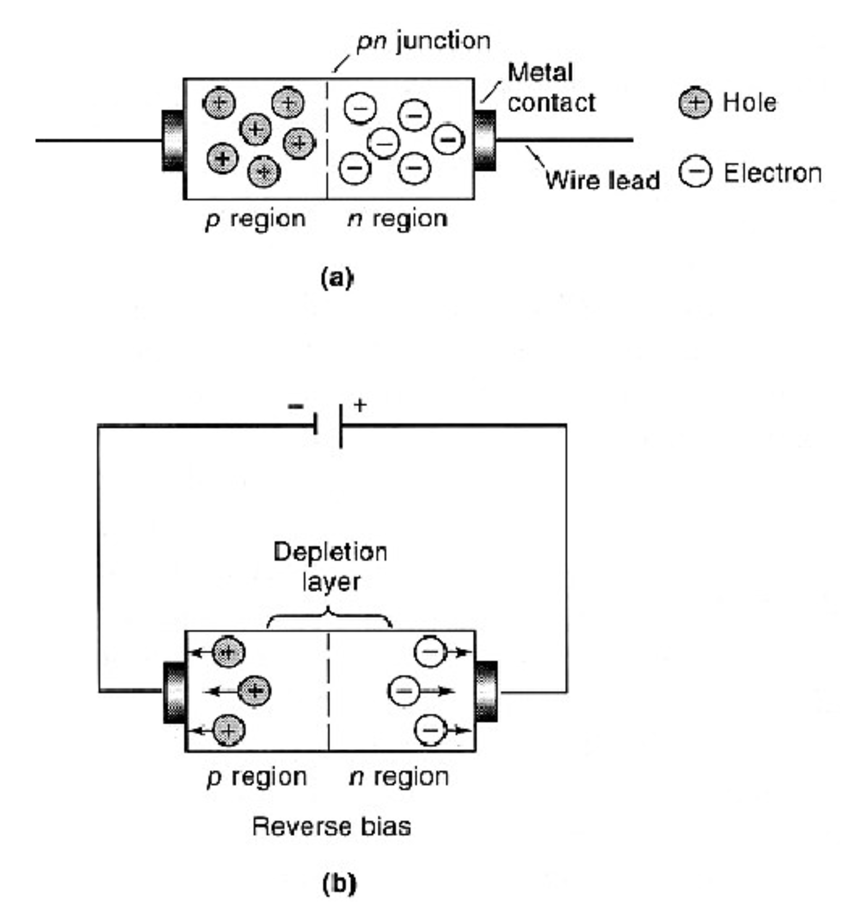
\includegraphics[scale=.25]{img/depletion.png}
  \caption{$p$-$n$ junction}
  \label{chain}
\end{figure}

\bigbreak

In intrinsic silicon there are $\sim 10^9$ free charge carriers at room
temperature but only $\sim 2 \times 10^4$ electrons are induced by a MIP
traversing 300 $\mu$m. Therefore a MIP signal would be lost among the large
number of free charge carriers. The operation of silicon detectors requires
sensors to be fully or partially depleted of free charge carriers. This can
be achieved by using $p$-$n$ junctions operated in reverse bias. Silicon sensors
are often fabricated on $n$-type bulk by adding a type V material, like
phosphorus \ce{P} (donor impurity) to silicon. Donor impurities provide an
excess of electrons charge carriers. Similarly a $p$-type material can be
realized by adding type III material like boron \ce{B} (acceptor impurities)
that yields an excess of holes as majority charge carriers. Typical doping
concentration used in $n$-bulk silicon sensors are of the order of
$1012$ cm$^{-3}$. The full depletion voltage V$_{\textup{FD}}$=D/2$\varepsilon
\mu \zeta$ depend on the thickness D, the resistivity $\varepsilon$, the
carrier mobility $\mu$, and the shape of the junction $\zeta$.

\bigbreak

\subsection{TRACE detector}

The TRacking Array for light Charged particle Ejectiles (TRACE) is a silicon
detector designed for fusion-evaporation and direct nuclear reactions.
The material, the thickness, the segmentation and a basic geometry have been
simply estimated by empirical considerations, while the final prototype was
chosen among the various geometries by the simulation of their performances
and comparison with already existing detector ancillaries (EUCLIDES, MUST2,
TIARA).

\bigbreak

\begin{figure}[h]
  \centering
  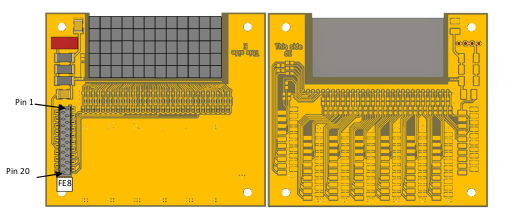
\includegraphics[scale=.65]{img/trace_e.png}
  \caption{TRACE detector (E configuration)}
  \label{chain}
\end{figure}

\begin{figure}[h]
  \centering
  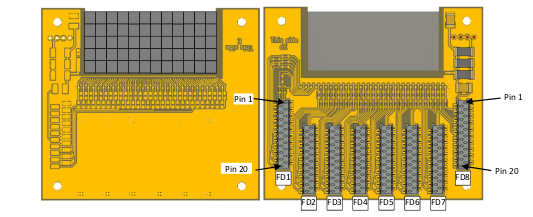
\includegraphics[scale=.65]{img/trace_de.png}
  \caption{TRACE detector (dE configuration)}
  \label{chain}
\end{figure}

\bigbreak

Silicon, for its transparency, energy resolution, moderate cost and
well known properties is chosen as a good compromise for the required
applications. Based on the efficiency criterion, particles dynamics ($\sim$
$100$ MeV for alpha particles and $25$ MeV for protons) and technological
constraints, the thickness of the detector has been chosen to be $150$ $\mu$m
and $1.5$ mm for the $\Delta$E and E layers respectively. The $4 \times 4$ mm
60 pad segmentation has been established from the requirement to have a uniform
counting rate ($20$ kHz maximum) when using high intensity beams and a good
angular resolution ($\sim 2^\circ$), necessary to perform momentum
discrimination in transfer reactions and a good Doppler correction. The pad
has been preferred to the strip segmentation due the expected smaller
electronics noise.

\subsection{Testing the TRACE detector}

In order to test the TRACE detector, it was put in a vacuum chamber, with a $\alpha$-ray source.

\subsection{GALTRACE experiment}

The experiment was performed in July 2019 at the Legnaro National Laboratory
(Italy). A \ce{^13C} beam, with energy of $23$ MeV and intensity around $1$ pnA
was focused on a $0.1$ mg/cm thick \ce{^19 F} -\ce{^7 Li} -\ce{^12 C} target.
Two TRACE silicon detectors were placed inside the GALILEO HPGe array
scattering chamber. A common electrode covered the entire ohmic side of the
detector.

\bigbreak

Inside the chamber, the detectors were connected with a short cable to a
16-channel charge-sensitive preamplifier, designed at INFN Milano~\cite{strano}.
The preamplifier gain was $45$ mV/MeV yeliding a dynamic range of
approximately 100 MeV. The trigger of the acquisition was the signal from the
common electrode. The signals from one detector were sent to the digital
acquisition, while the second detector was connected to the analog read-out
line.

\bigbreak

The chain of the digital acquisition allowed to collect the signals (“traces”)
digitized by the 100 MHz sampling module. The length of the recorded trace was
1 $\mu$s, giving 100 points, at every 10 ns each. This length of the traces
was chosen to assure recording the full rise time on the one hand and at the
same time minimize the amount of written data. The signals were recorded,
digitized and afterwards processed to extract the relevant observables. The
placement of the TRACE module in the chamber with the ohmic side facing the
reaction products was important to enhance the PSA capability. The signals
were collected both from the ohmic side of the detector as well as from a few
groups of pads (or single pads).

\bigbreak

The trigger of the TRACE acquisition, obtained in this case from a digital
leading edge discriminator embedded in the module, was the signal from the
common electrode (“BACK”). The signals from the pads were collected only if
the BACK signal was present.